\documentclass[a4paper, 12pt]{article}

%Абзацный отступ

\usepackage{indentfirst}

%Рисунки

\usepackage{graphicx}
\usepackage{wrapfig}

%Гиперссылки и работа с цветом

\usepackage{hyperref}
\usepackage[rgb]{xcolor}
\hypersetup{			%Гиперссылки
	colorlinks=true, 	%false: ссылки в рамках
	urlcolor=blue		%на URL
}

%Русский язык

\usepackage[T2A]{fontenc}		%кодировка
\usepackage[utf8]{inputenc}		%кодировка исходного текста
\usepackage[english, russian]{babel}	%локализация и переносы


%Математика

\usepackage{amsmath, amsfonts, amssymb, amsthm, mathtools, mathrsfs}

\author{Штрайх Роберт}
\title{Работа 3.3.4. Эффект Холла в полупроводниках}
\date{28 сентября 2021 г.}

\begin{document}
\begin{titlepage}
	\centering
	\vspace{5cm}
	{\scshape\LARGE Московский физико-технический институт \par}
	\vspace{4cm}
	{\scshape\Large Лабораторная работа №3.3.4 \par}
	\vspace{1cm}
	{\huge\bfseries Эффект Холла в полупроводниках \par}
	\vspace{1cm}
	\vfill
\begin{flushright}
	{\Large выполнил студент 006 группы ФЭФМ}\par
	\vspace{0.3cm}
	{\Large Штрайх Роберт}
\end{flushright}
	

	\vfill

% Bottom of the page
	Долгопрудный, 2021 г.
\end{titlepage}

\newpage
\textbf{Цель работы:} измерение подвижности и концентрации носителей заряда в полупроводниках.

\textbf{В работе используются:} электромагнит с регулируемым источником питания; вольтметр; амперметр; миллиамперметр; милливеберметр или миллитесламетр; источник питания (1,5 В), образцы легированного германия.

\section{Теоретические сведения}

Во внешнем магнитном поле \textbf{\textit{B}} на заряды действует сила Лоренца:

\begin{equation} \label{Lorens}
\textbf{\textit{F}} = q\textbf{\textit{E}} + q\textbf{\textit{u}} \times \textbf{\textit{B}}.
\end{equation}
Эта сила вызывает движение носителей, направление которого в общем случае не совпадает с \textbf{\textit{E}}. Возникновение поперечного тока электрического поля в образце, помещённом во внешнее магнитное поле, называют \textit{эффектом Холла.}

В работе изучаются особенности проводимости проводников в геометрии \textit{мостика Холла}. Ток пропускается по плоской полупроводниковой пластинке, помещённой в перпендикулярное пластинке магнитное поле. Измеряется разность потенциалов между краями пластинки в поперечном к току направлении. По измерениям определяется \textit{константа Холла}, тип проводимости (\textit{электронный} или \textit{дырочный}) и на основе соотношения \eqref{R_x} вычисляется концентрация основных носителей заряда.

\section{Расчётные формулы}

\begin{itemize}
\item ЭДС Холла:
\begin{equation} \label{E}
\mathscr{E_\text{х}} = U_{34} - U_0,
\end{equation}
\item Постоянная Холла:
\begin{equation} \label{R_x}
R_x = -\frac{\mathscr{E_\text{х}}}{B}\cdot\frac{a}{I} = \frac{1}{nq},
\end{equation}
\item Концентрация носителей тока в образце:
\begin{equation} \label{n}
n = \frac{1}{R_xe},
\end{equation}
\item Удельная проводимость материала образца:
\begin{equation}
\sigma = \frac{IL_{35}}{U_{35}al},
\end{equation}
\item Подвижность носителей тока:
\begin{equation}
b = \frac{\sigma}{en}.
\end{equation}
\end{itemize}

\section{Экспериментальная установка}

\begin{figure}[h]
\begin{center}
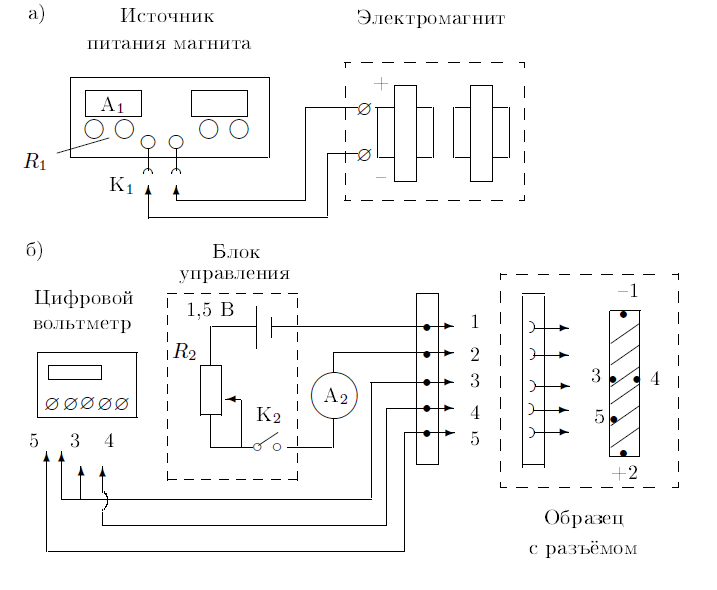
\includegraphics[width=1\textwidth]{Рисунок_установки}
\end{center}
\caption{Схема установки для исследования эффекта Холла в полупроводниках}
\end{figure}
\end{document}

